\subsection{Fluctuations of conserved charges} 
\subsubsection{Physics introduction and observables}

Generally, fluctuations can be linked to critical behavior associated with a phase transition. In the phase diagram of strongly interacting matter at zero net baryon density, presence of a chiral phase transition between hadronic matter and QGP has been conjectured \cite{Pisarski:1983ms}, and arguments have been presented~\cite{Ejiri:2009ac,Ding:2018auz} in lattice QCD (lQCD) that the transition, for vanishing light quark masses, is of second order and belongs to the O(4) universality class. Due to the small but finite physical quark masses, in lQCD a rapid cross over is found \cite{Aoki:2006we,Aoki:2009sc,Borsanyi:2010bp,Bazavov:2011nk,Bhattacharya:2014ara}   which, however, exhibits pseudo-critical features due to the smallness of the u- and d-quark masses and the proximity of the cross over region to the O(4) line \cite{Ejiri:2009ac,Ding:2013lfa}. It has been pointed out that, in order to test the critical behavior linked to the phase diagram of strongly interacting matter, fluctuations of conserved charges can provide an experimental observable \cite{Ejiri:2005wq,Bazavov:2017dus,Friman:2011pf,Bazavov:2012jq}. Generally, these fluctuations can be linked to susceptibilities, more concretely to the derivatives of the pressure with respect to the various chemical potentials linked to the conserved charges. The 'charges' here are baryon number B, strangeness S, and electrical charge Q. These so-called generalized susceptibilities can be computed in lQCD at vanishing chemical potential, i.e. exactly for the situation probed with experiments at the LHC. They are defined (see e.g. \cite{Bazavov:2012jq,Bellwied:2015lba}) in terms of dimensionless normalized chemical potentials \(\hat{\mu}_X\equiv \mu_X/T \) \: as

\begin{equation}
\chi_{ijk}^{BQS}(T) = \left.
\frac{\partial P(T,\hat{\mu})/T^4}{\partial\hat{\mu}_B^i \partial\hat{\mu}_Q^j \partial\hat{\mu}_S^k}\right|_{\hat{\mu}=0} \; .
\label{suscept}
\end{equation} 

\noindent Experimentally, these generalized susceptibilities can, for conserved 'charges' such as the net number of baryons, be related to fluctuations of the conserved charges. For instance, a measurement of higher moments or cumulants of net baryon number in relativistic nuclear collisions can then be directly related \cite{Karsch:2010ck,Skokov:2012ds,Karsch:2012wm,Karsch:2017mvg,Borsanyi:2013hza,Borsanyi:2014ewa} to theoretical predictions from lQCD or from more phenomenological models  of the chiral phase transition  \cite{Almasi:2017bhq,Parotto:2018pwx}  to shed light on the possible critical behavior near the QCD phase boundary. For a distribution $\Delta N_B$ of the net baryon number, $N_B - \bar{N_B}$, with moments defined as 

\begin{equation}
\mu_i = \langle (\Delta N_B - \langle \Delta N_B \rangle )^i \rangle ,
\end{equation}
the cumulants $\kappa_i$ can be directly linked to the generalized susceptibilities such as

\begin{equation}
\kappa_2 = \mu_2 = VT^3 \chi_2^B
\end{equation}
\begin{equation}
\kappa_3 = \mu_3 = VT^3 \chi_3^B  
\end{equation}

\begin{equation}
\kappa_4 = \mu_4 - 3\mu_2^2 = VT^3 \chi_4^B.
\end{equation}


\begin{figure}[h]
\begin{center}
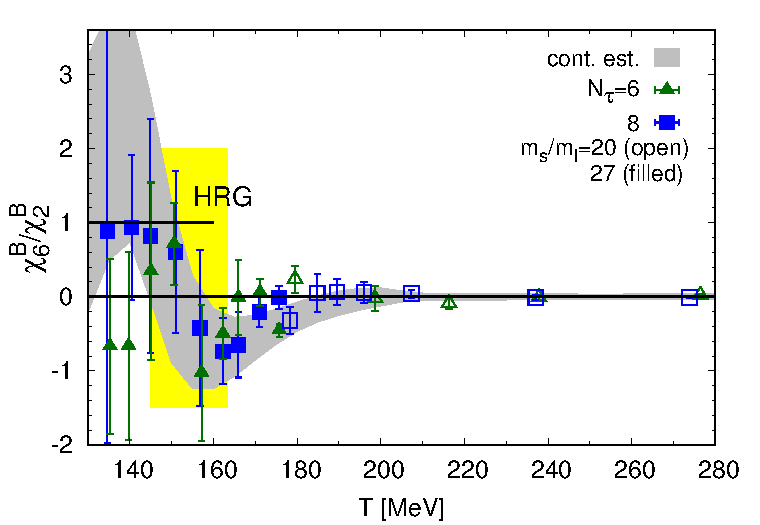
\includegraphics[width=0.45\textwidth]{\main/lightflavour/figs/B6_B2_wideT_27.pdf}
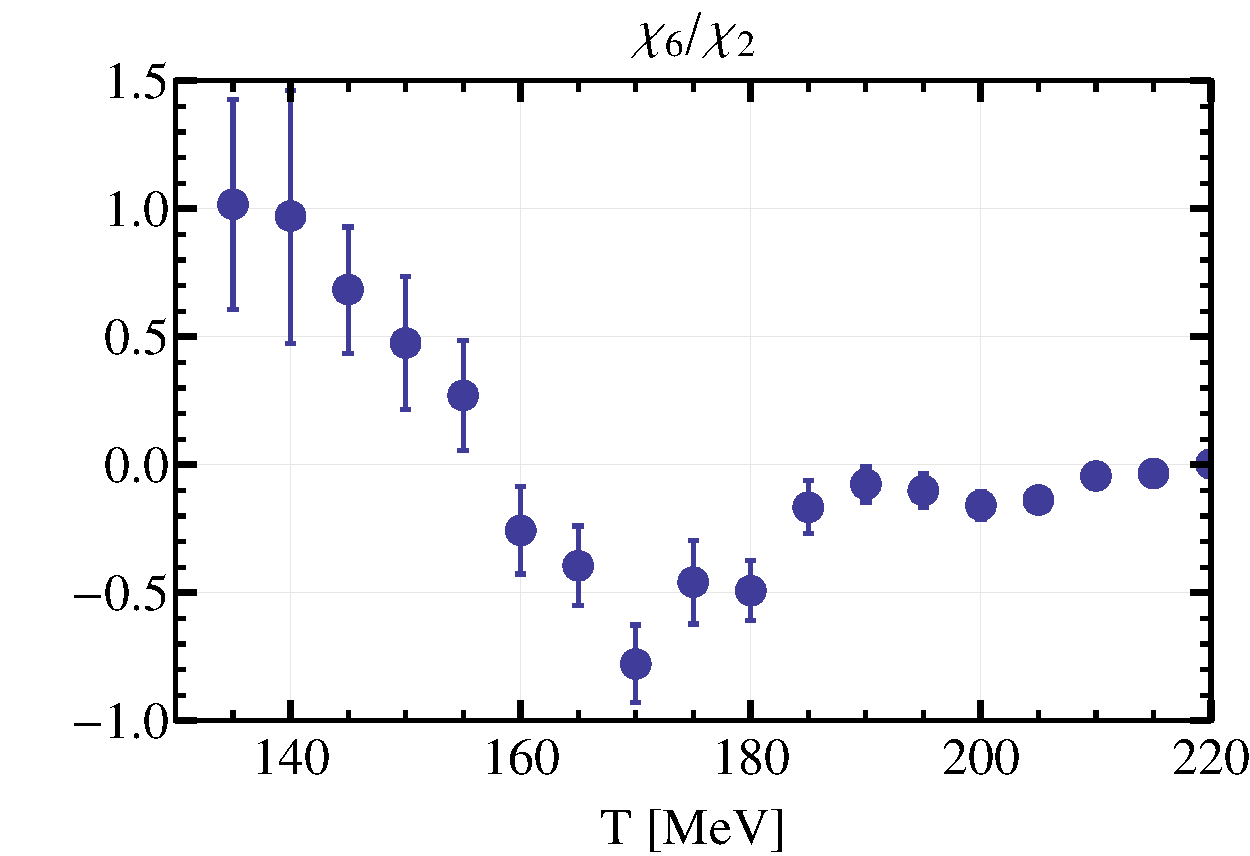
\includegraphics[width=0.46\textwidth]{\main/lightflavour/figs/c6c2_fromLattice.pdf}
\end{center}
\caption{Ratio of 6th to 2nd order baryon number susceptibility from lQCD. The left-hand figure is from Ref. \cite{Bazavov:2017dus}. The right-hand figure is calculated  from recent lQCD data on  6th and  2nd  order susceptibility from Ref.  \cite{Borsanyi:2018grb}.  }  
\label{fig:chi62}
\end{figure}

In the O(4) universality class a singular contribution to the pressure shows up for higher order  moments.
More specifically, at vanishing chemical potential, all odd susceptibilities of the net baryon number vanish.  In addition, in the O(4) universality class, the second and fourth order susceptibilities remain finite  at  the  phase  transition  temperature  at $\mu_B=  0$  in  the  chiral  limit,
implying  that  only  sixth  and  higher  order  susceptibilities  diverge \cite{Ejiri:2005wq,Friman:2011pf}. Thus, for  physical  quark  masses and at $\mu_B=0$,  only  higher  order  cumulants $\kappa_n$ with $n\geq 6$ can exhibit   O(4) criticality,  whereas at finite $\mu_B$ this is already the case for $\kappa_n$ with $n\geq 3$.  

Sensitivity to chiral criticality due to the vicinity of the O(4) line    at $\mu_B=0$ is borne out for phenomenological models as is shown in \cite{Friman:2011pf,Almasi:2017bhq}, or for lQCD predictions \cite{Bazavov:2017dus,Borsanyi:2018grb} by strong deviations of $\chi_6^B/\chi_2^B$ from unity as shown in figure~\ref{fig:chi62}.

We note that a convenient baseline for the expected values of cumulants of distributions/fluctuations of produced particles in relativistic nuclear collisions can be obtained in the framework of the hadron re\-so\-nance gas \cite{Allton:2005gk,Karsch:2010ck,BraunMunzinger:2011ta,Borsanyi:2018grb,Luo:2017faz}. There, Poissonian fluctuations lead to moments and cumulants for net baryon number which all can be expressed in the following way \cite{BraunMunzinger:2011ta,BraunMunzinger:2011dn, Braun-Munzinger:2018yru}:
\begin{equation}
\label{lbaseline}
\kappa_n(N_B - N_{\bar B}) = \langle (N_B +(-1)^n N_{\bar{B}}) \rangle
\end{equation}
For zero net baryon number then all odd cumulants vanish and all even cumulants are identical.

Measuring such cumulants with precision poses a formidable experimental challenge due to the requirement of very large data sets ($> 10^9$ events of a particular event or centrality class) with superb control of systematic uncertainties. In addition, non-critical contributions to the cumulants from volume fluctuations and global baryon number conservation \cite{Skokov:2012ds,Braun-Munzinger:2016yjz, Braun-Munzinger:2018yru} need to be evaluated and the data accordingly corrected. Furthermore, in particular for comparison to lQCD predictions, care needs to be taken to keep experimental cuts such as in p$_T$ to a minimum as such cuts cannot be introduced in lQCD \cite{Karsch:2015zna,Alba:2015iva}.
     
\subsubsection{State of the art from experiments and present limitations}
Fluctuations of net-protons, measured by the STAR and ALICE experiments provided interesting and stimulating results. The measurements at STAR complement the corresponding measurements from ALICE, which allows to pin down the global structure of the phase diagram of strongly interacting matter in the wide range of temperatures and net-baryon densities. However, before drawing firm conclusions, by e.g., confronting with the theoretical calculations, non-dynamical contributions stemming from unavoidable fluctuations of  participant nucleons and  overall baryon number conservation have to be subtracted from the experimental measurements. Both of these non-dynamical contributions, which exist neither in lQCD no in HRG, led to deviations from the baseline as defined in Eq.~\ref{lbaseline}. Indeed, the acceptance dependence of the second order cumulants of net-protons, measured by ALICE~\cite{Rustamov:2017lio}, exhibits deviations from the non-critical baseline (cf. the left panel of Fig.~\ref{netpALICE_STAR}). However, these deviations were explained by the global baryon number conservation~\cite{Rustamov:2017lio, Braun-Munzinger:2016yjz, Braun-Munzinger:2018yru}, which, in accordance with the experimental findings, decreases the amount of fluctuations with the increasing acceptance. This is the first experimental verification of the lQCD predictions for the second order cumulants of net-baryon distributions. On the other hand, the energy dependence of $\kappa_{4}/\kappa_{2}$ of net-protons, measured by STAR, shows non-monotonic deviations from unity. As seen in the right panel of Fig.~\ref{netpALICE_STAR}, apart from the two lowest energies of $\sqrt{s_{NN}}$ = 7.7A and 11.5A GeV, the experimental measurements show increasing trend, ultimately approaching unity. Recently this  behavior was also explained by the presence of non-dynamical effects~\cite{Braun-Munzinger:2018yru}. Experimental measurements of net-proton moments beyond the fourth order are necessary in order to disentangle dynamical fluctuations from those originating from non-dynamical effects.

As mentioned in the previous section, even at vanishing net-baryon densities, lQCD calculations predict critical fluctuations encoded in the temperature dependence of $\kappa_{4}/\kappa_{2}$ and $\kappa_{6}/\kappa_{2}$. This motivates our experimental program  of measuring higher moments of net-proton distributions at the LHC energies. 

\begin{figure}[h]
\begin{center}
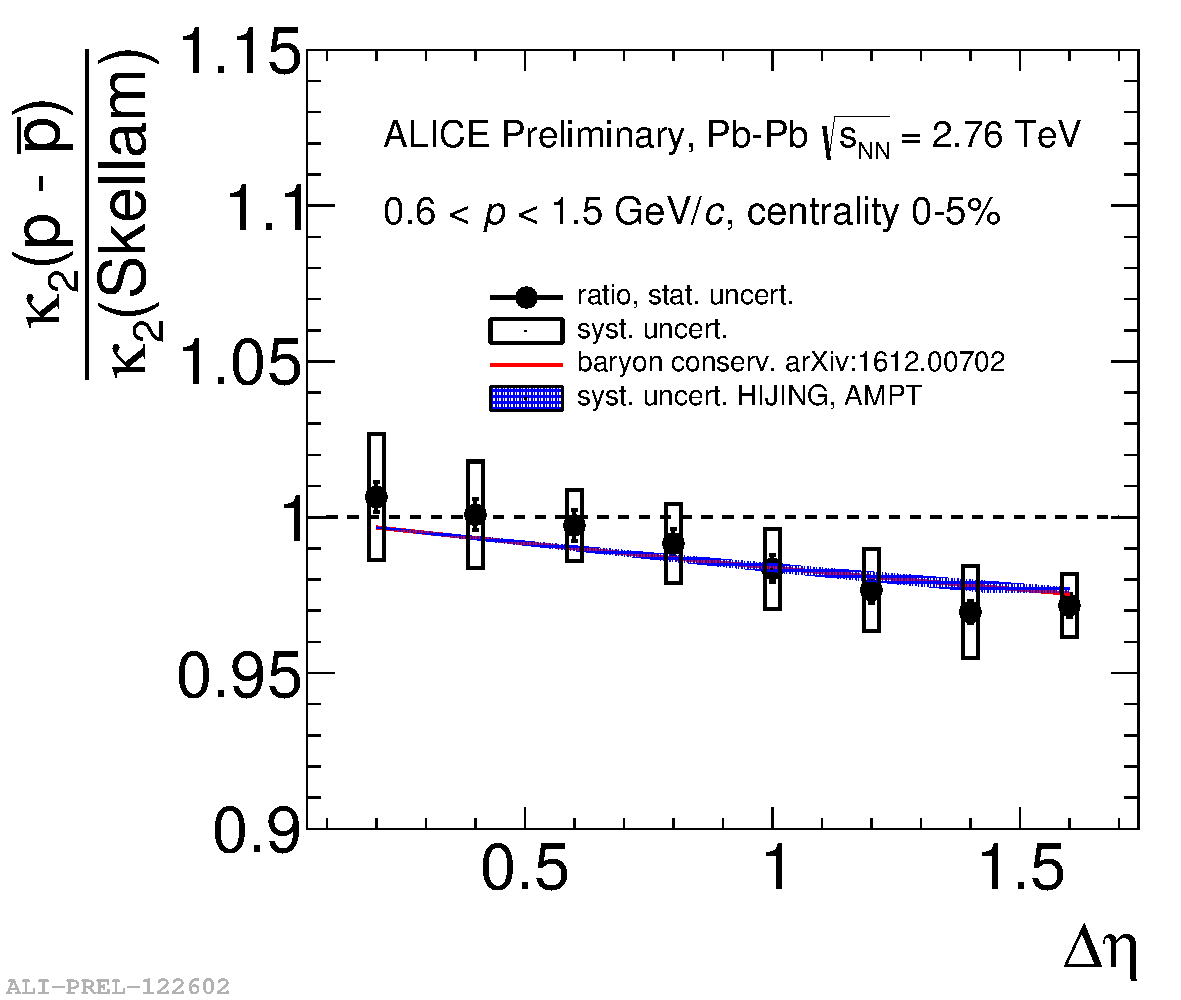
\includegraphics[width=0.53\textwidth]{\main/lightflavour/figs/2017-Feb-03-rapProton1.pdf}
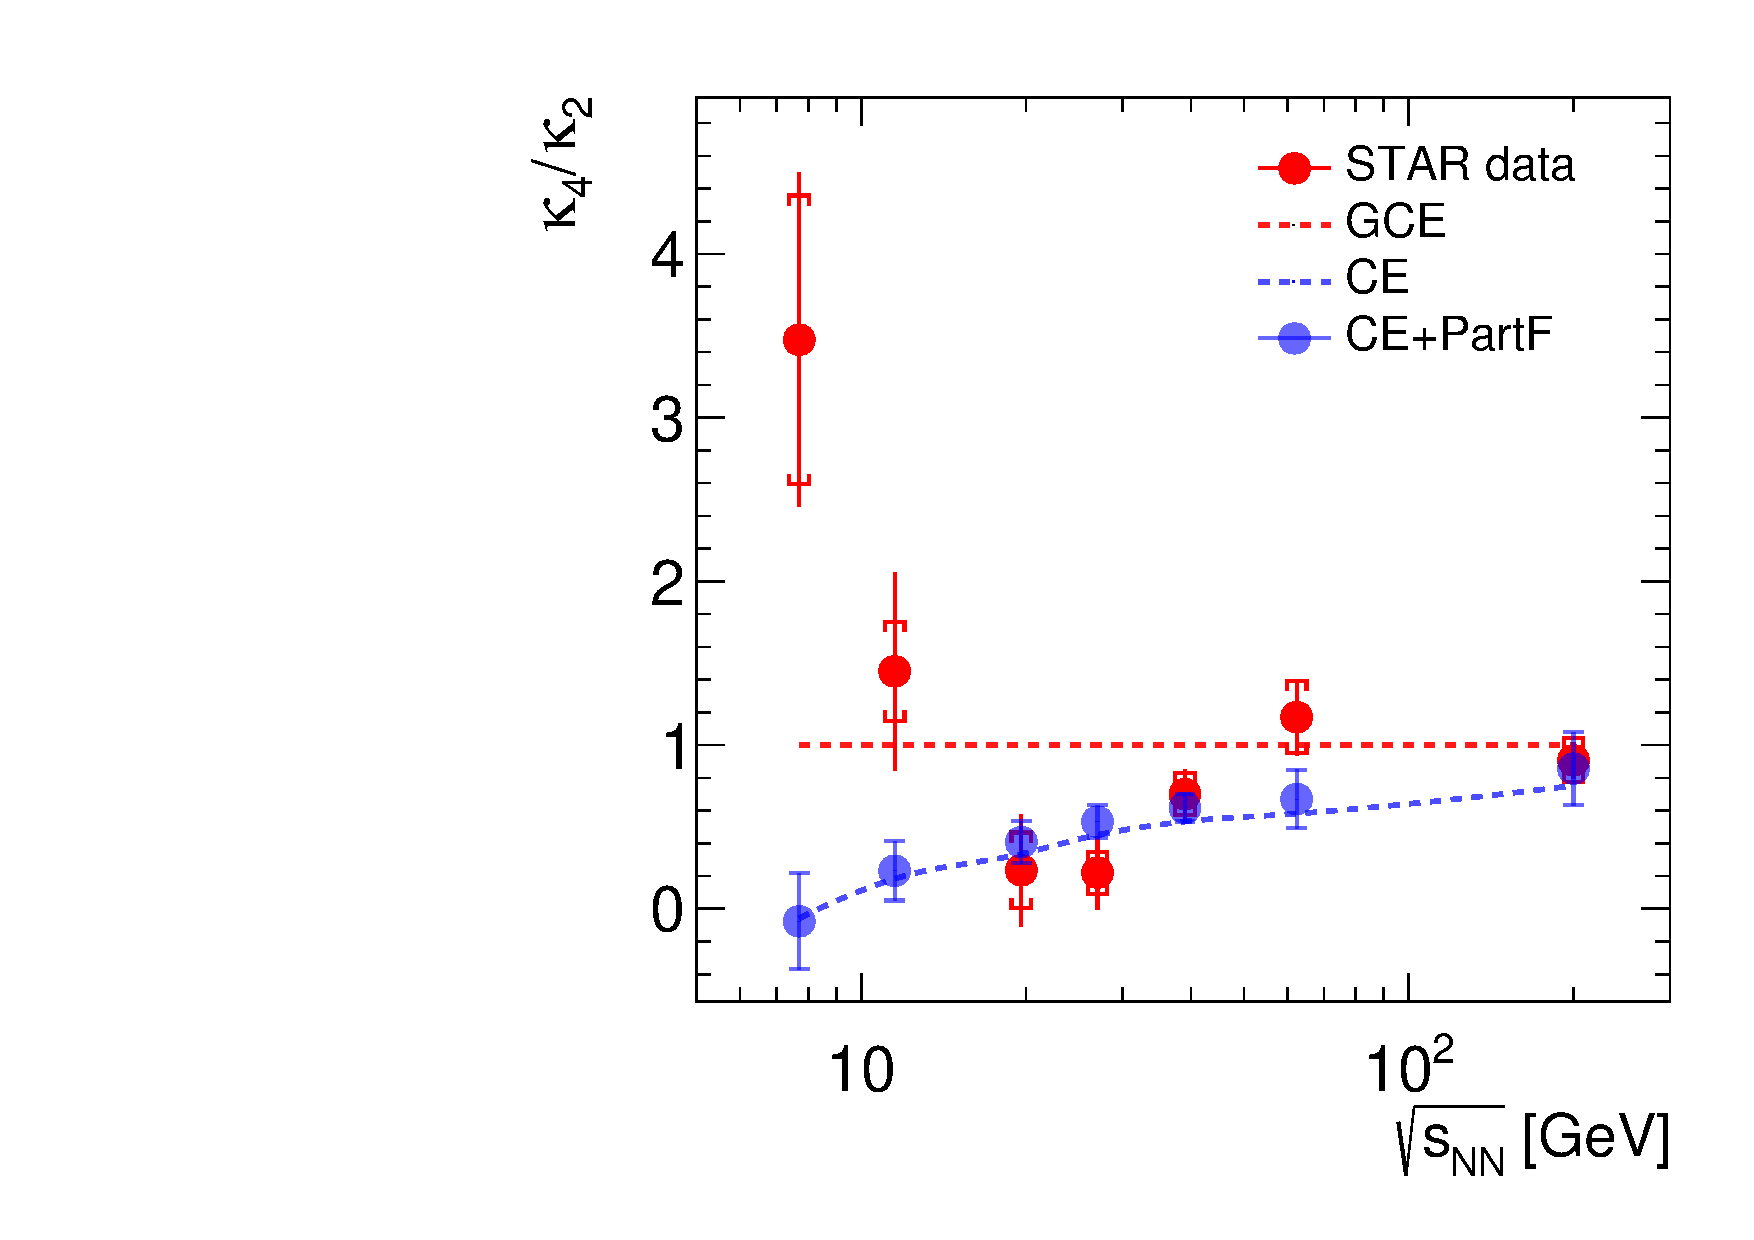
\includegraphics[width=0.46\textwidth]{\main/lightflavour/figs/k4k2QM18.pdf}
\end{center}
\caption{\textcolor{blue}{Placeholder, to be updated.} Left panel: Pseudorapidity dependence of the normalised second order cumulants of net-protons as measured by the ALICE collaboration~\cite{Rustamov:2017lio}. The red solid line shows the effect of the baryon number conservation. Right panel: $\kappa_{4}/\kappa_{2}$ measurements from STAR (the red circles) compared to predictions from non-critical fluctuations (the blue symbols)~\cite{Braun-Munzinger:2018yru}. The blue dashed line corresponds the non-critical fluctuations without participant fluctuations. The red dashed line represents the GCE baseline.}  
\label{netpALICE_STAR}
\end{figure}



\subsubsection{Projections for LHC Run3 and 4}
Precise measurement of higher order cumulants are needed to constrain the lattice QCD predictions as discussed in the previous section. However, study of higher order cumulants of net-particle distributions are of statistics hunger in nature. Therefore, a toy MC simulation is carried out to project the required event statistics for the measurements of higher order cumulants of net-proton. As the main motivation is to measure the ratio of cumulants, this MC study is focused only on the results of $\mathrm{\kappa}_{4}/\mathrm{\kappa}_{2}$ and $\mathrm{\kappa}_{6}/\mathrm{\kappa}_{2}$. The basic structure of the toy MC study is as follows. Independent proton (p) and anti-proton ($\mathrm{\bar{p}}$) distributions are considered to get the net-proton distributions. To model the p and $\mathrm{\bar{p}}$ multiplicity distributions, Pearson curve method (PCM) is used \cite{Behera:2017xwg}. In PCM, the first four cumulants are used as input to construct the probability distribution functions (PDF).  The first four cumulants values of p and $\mathrm{\bar{p}}$ are taken from the analysis presented in Ref. \cite{Behera:2018wqk}. In this study, the results of most central events of Pb--Pb collisions at $\sqrt{s_{\mathrm{NN}}}$ = 2.76 TeV are used.

The statistical uncertainties depend on the reconstruction efficiencies of particles \cite{Luo:2017faz}. Hence, instead of looking at generated event samples, the statistical uncertainties are estimated for the efficiency-corrected sample. For a realistic approach, the p and $\mathrm{\bar{p}}$ numbers are generated randomly from their PDFs. Each particles are assigned by a transverse momentum ($p_{T}$) following the shape of ALICE p ($\mathrm{\bar{p}}$) spectra \cite{Abelev:2013vea}. A $p_{T}$ dependent reconstruction efficiency ($\sim 65\%$ for p and $\sim 60\%$ for $\mathrm{\bar{p}}$) is applied to each generated particles. They are labeled as the reconstructed sample. To estimate the efficiency corrected net-proton $\mathrm{\kappa}_{4}/\mathrm{\kappa}_{2}$ and $\mathrm{\kappa}_{4}/\mathrm{\kappa}_{2}$, the same analysis framework and method are used as in Ref. \cite{Behera:2018wqk}. The simulation is carried out for different event statistics. Furthermore, for each set of event statistics, 5 different samples are generated by changing the pseudo-random numbers. The $\mathrm{\kappa}_{4}/\mathrm{\kappa}_{2}$ and its statistical uncertainties are shown in Figure \ref{fig:c4c2toymc} (a) as a function of event statistics. The dashed line in the upper panel corresponds to the analytically estimated value of $\mathrm{\kappa}_{4}/\mathrm{\kappa}_{2}$ from the net-proton distribution ($f(\Delta \mathrm{p}) = f(\mathrm{p}) - f(\mathrm{\bar{p}})$). 


\begin{figure}[h]
\begin{center}$
\begin{array}{cc}
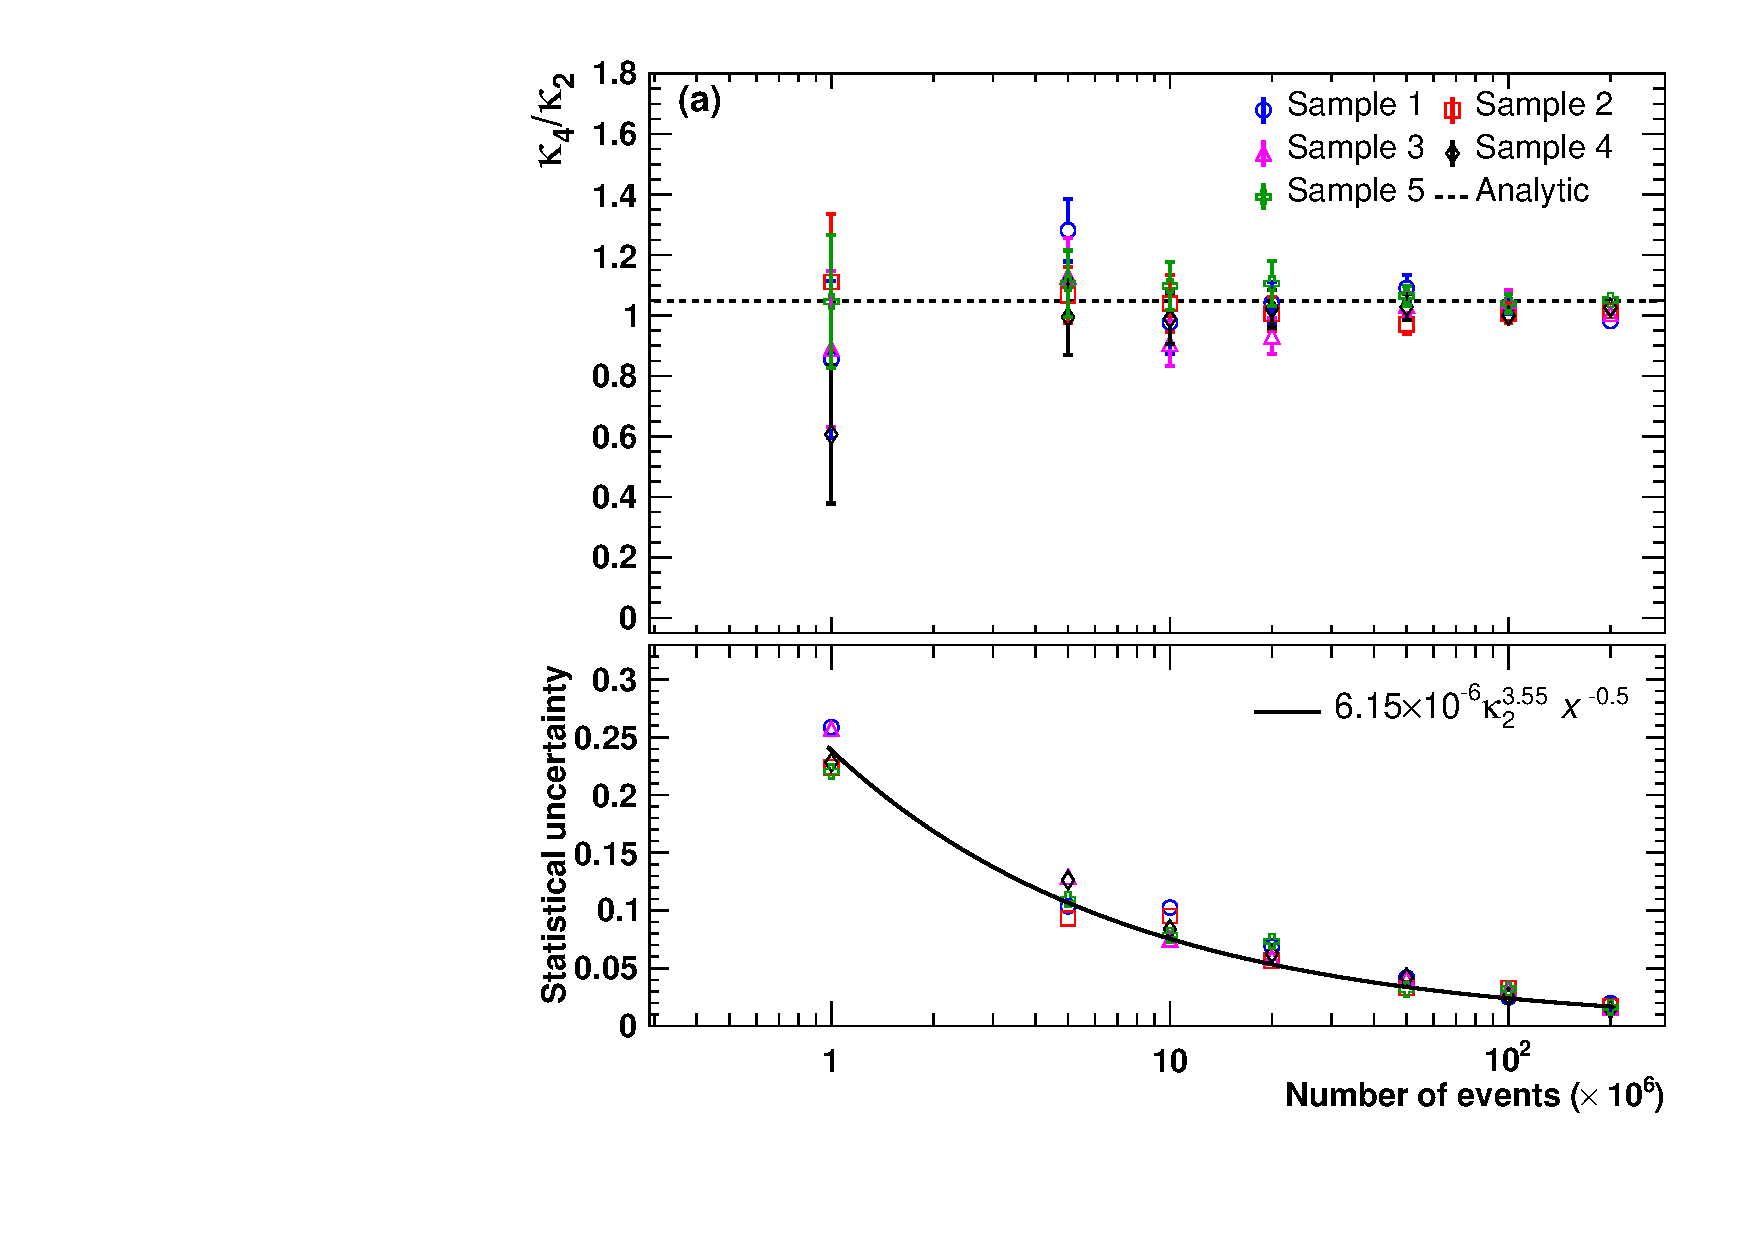
\includegraphics[width=0.45\textwidth]{\main/lightflavour/figs/NetProtonC4C2wErr.pdf} &
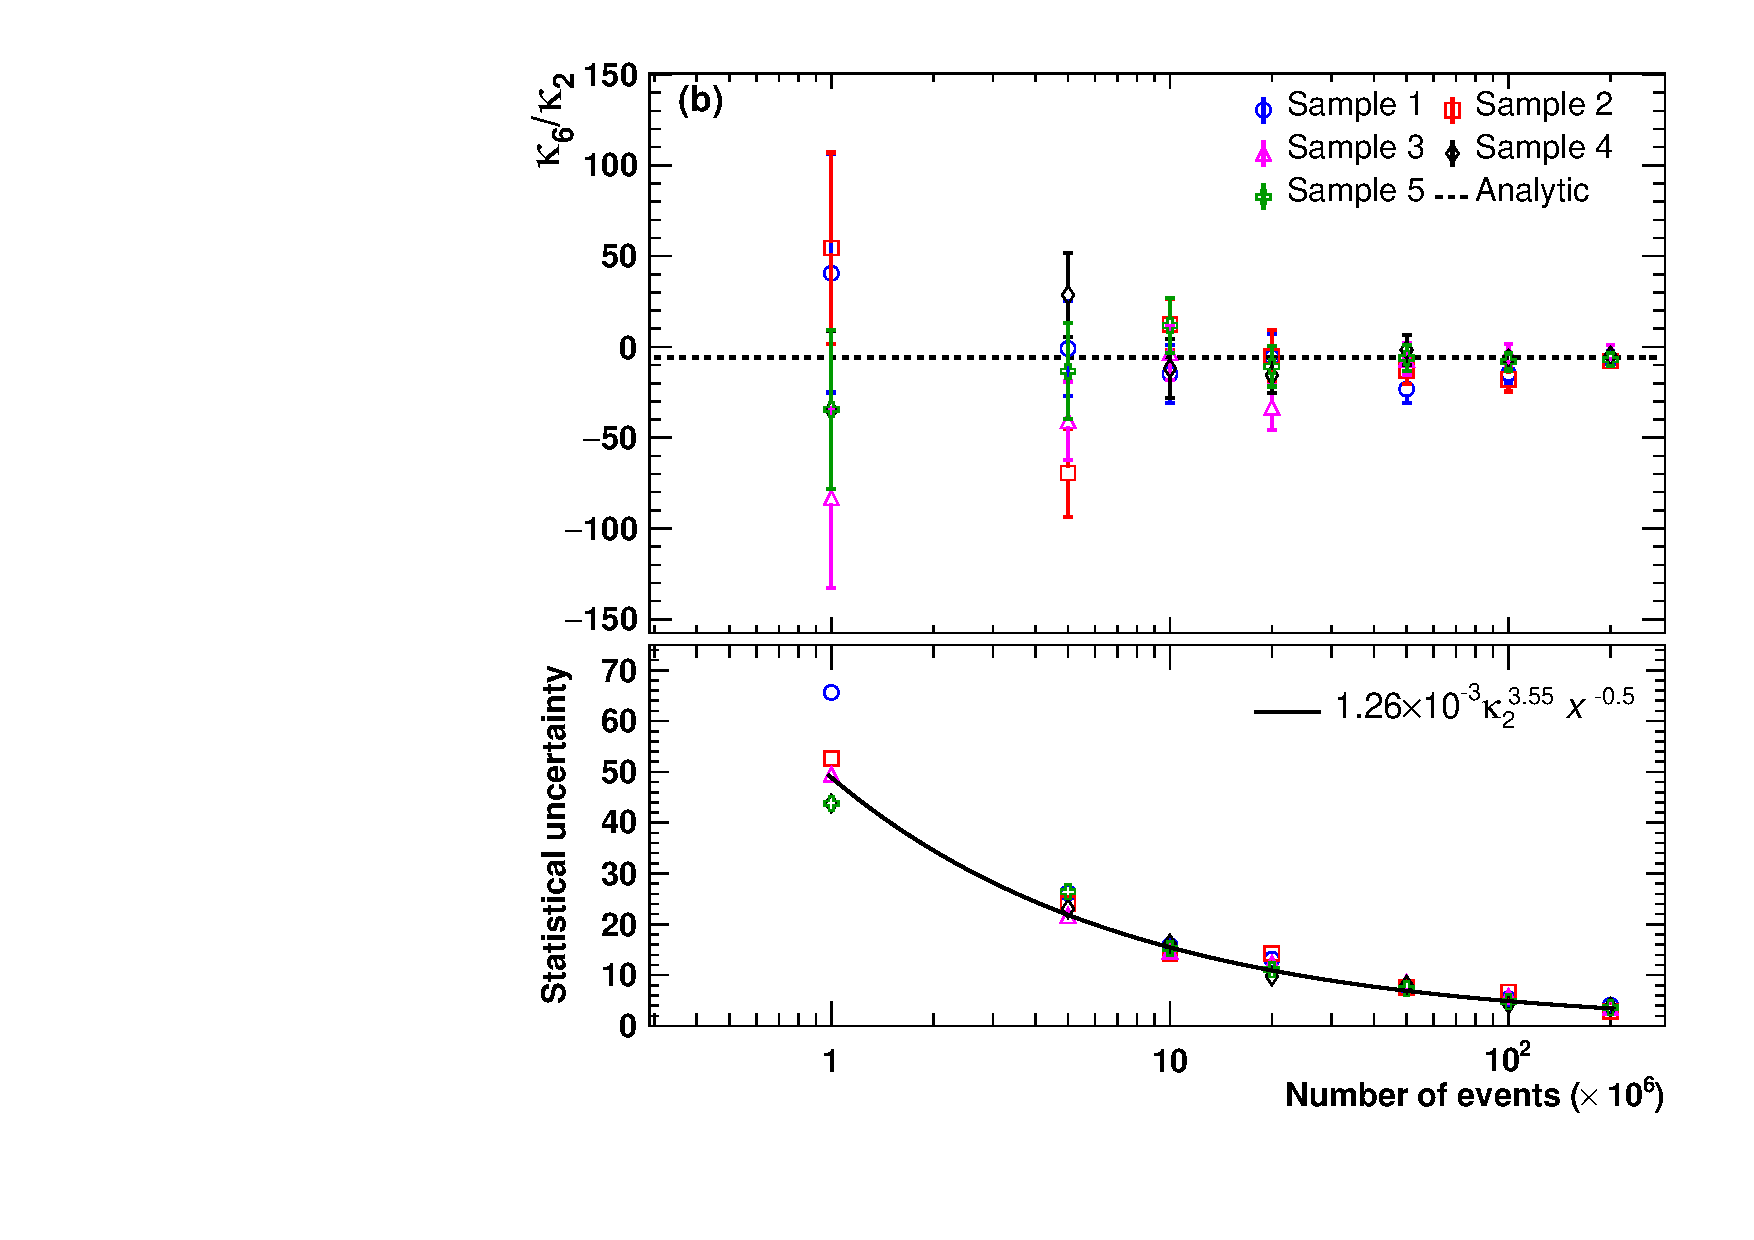
\includegraphics[width=0.45\textwidth]{\main/lightflavour/figs/NetProtonC6C2wErr.pdf}
\end{array}$
\end{center}
\caption{\textcolor{blue}{Placeholder, to be updated.} (a) $\mathrm{\kappa}_{4}/\mathrm{\kappa}_{2}$ of net-proton distributions in most central Pb--Pb collisions are shown for different event statistics. The statistical uncertainty of $\mathrm{\kappa}_{4}/\mathrm{\kappa}_{2}$ for different event statistics are shown in the lower panel. The results are shown for 5 different samples as described in the text. The dashed line represents the analytical value of $\mathrm{\kappa}_{4}/\mathrm {\kappa}_{2}$ of net-proton distributions. (b) $\mathrm{\kappa}_{6}/\mathrm {\kappa}_{2}$ of net-proton distributions in most central Pb--Pb collisions are shown for different event statistics. The statistical uncertainty of $\mathrm{\kappa}_{6}/\mathrm{\kappa}_{2}$ for different event statistics are shown in lower panel. The results are shown for 5 different samples as described in the text. The dashed line in the upper panel represents the analytical value of $\mathrm{\kappa}_{6}/\mathrm{\kappa}_{2}$ of net-proton distributions. The solid lines in the lower panel of Figure (a) and (b) are parametrised function of $\mathrm{\kappa_{2}}$ and event numbers in the unit of $10^{6}$}
\label{fig:c4c2toymc}
\end{figure}


Similarly, in Figure \ref{fig:c4c2toymc} (b), the efficiency corrected results of $\mathrm{\kappa}_{6}/\mathrm{\kappa}_{2}$ and the statistical uncertainties for different event statistics are shown in the upper and lower panel, respectively. The dashed line in the top panel represents the analytical value of net-proton $\mathrm{\kappa}_{6}/\mathrm{\kappa}_{2}$. It can be seen from the Figure \ref{fig:c4c2toymc} (a) and (b), with increasing event statistics the $\mathrm{\kappa}_{4}/\mathrm {\kappa}_{2}$ and $\mathrm{\kappa}_{6}/\mathrm{\kappa}_{2}$ results converge towards the analytical value. Moreover, the statistical uncertainties are also decreased with increasing event statistics. It is observed that at 200$\times 10^{6}$ of events, the relative statistical uncertainty on $\mathrm{\kappa}_{4}/\mathrm {\kappa}_{2}$ is less than 2$\%$. At the same event statistics, the relative statistical uncertainty on $\mathrm{\kappa}_{6}/\mathrm{\kappa}_{2}$ is around 30-40$\%$. From this study, it is evident that for less than 500$\times 10^{6}$ events will be enough for $\mathrm{\kappa}_{4}/\mathrm {\kappa}_{2}$ measurement of net-proton with less than 1$\%$ statistical uncertainty in most central Pb--Pb collisions. However, for more precise measurements of $\mathrm{\kappa}_{6}/\mathrm {\kappa}_{2}$, one needs more than $10^{9}$ of events only in most central Pb--Pb collisions, which is in the reach of Run3 and Run4. Additionally, it should be noted that this MC study is done for the data in a relatively smaller $p_{T}$ window ($0.4 < p_{T} < 1.0$ GeV/$c$). With increasing $p_{T}$ range up to 2 GeV/$c$, the width of the net-proton distribution will increase. In that case, the requirement of event statistics will be more (roughly 10 times).
 
%\subsubsection{Complementarity with other facilities}

\subsubsection{Diffusion of net baryon number, electric charge etc. and how to constrain it}
In a fluid dynamic description of heavy ion collisions, conserved (or almost conserved) quantum numbers have evolution equations governed by an interplay of conservation laws and local diffusion. For example, the local net baryon number density $n(\tau, x, y, \eta)$ as a function of Bjorken time $\tau$, transverse coordinates $x,y$ and rapidity $\eta$ is for a Bjorken-type expansion, and in a first-order approximation to relativistic fluid dynamics, governed by the following evolution equation,
\begin{equation}
\partial_\tau n + \frac{1}{\tau}n - D(\tau) \left( \partial_x^2 + \partial_y^2 + \frac{1}{\tau^2} \partial_\eta^2 \right) n =0.
\end{equation}
(This diffusion law is somewhat modified in a causal, second order approximation but this is a minor point for the following arguments.) While the term $\sim 1/ \tau$ describes simply the dilution due to the overall expansion of the system, the term $\sim D$ describes baryon diffusion. The baryon diffusion constant $D$ is a fundamental transport property of the quark-gluon plasma, similar to shear viscosity $\eta$ or bulk viscosity $\zeta$. In fact, it is directly related to heat conductivity $\kappa$ by the following relation
\begin{equation}
D = \kappa \left[ \frac{nT}{\epsilon + p} \right]^2 \left( \frac{\partial (\mu/T)}{\partial n} \right)_\epsilon,
\label{eq:baryondiffusionheatconductivity}
\end{equation}
where $n$ is the net baryon number and $\mu$ is the corresponding chemical potential. Equation \eqref{eq:baryondiffusionheatconductivity} seems to suggest that the diffusion constant $D$ vanishes in the limit $\mu\to 0$ (relevant to high energy collisions such at at LHC), but in fact theoretical calculations (both in the weak and strong coupling approximation) show that $\kappa$ is divergent $\sim 1/\mu^2$ so that $D$ is expected to be finite for $\mu\to 0$. It would be highly interesting to constrain the diffusion constant $D$ from experiments. This holds equally for related transport coefficients that come in for a second order approximation to relativistic fluid dynamics (in particular a relaxation time for the baryon diffusion current) and similar diffusion constants for net strangeness, charm etc. Diffusion of net electric charge is in a similar way determined by the electric conductivity and it is clear that it would be highly interesting to constrain it, as well.
It is clear that the local distribution of net baryon number on the freeze-out surface is reflected in the momentum space distributions and correlation functions that can be accessed experimentally. Experimental techniques and phenomenological theory need to be developed further but it is clear that differential correlation functions of net baryon number and other conserved quantum numbers are of high interest and should be measured as good as possible. For a more detailed discussion and further references see also [S. Floerchinger \& M. Martinez, Phys. Rev. C 92, 064906 (2015)].
The most direct example here is a two-point correlation function of net baryon number in momentum space \cite{Floerchinger:2015efa},
\begin{equation}
\frac{dN_\text{net-baryon,2}}{p_{T1} dp_{T1} p_{T2} dp_{T2}d\phi_1d\phi_2d\eta_1 d\eta_2} - \frac{dN_\text{net-baryon,1}}{p_{T1} dp_{T1} d\phi_1d\eta_1}  \frac{dN_\text{net-baryon,1}}{p_{T2} dp_{T2} d\phi_2d\eta_2}.
\end{equation}
This is essentially a weighted two-particle correlation function where each particle is weighted according to its net baryon number, i.\ e.\ weight $0$ for mesons, $+1$ for protons, $-1$ for anti-protons, $+3$ for $^3\text{He}$ ions and so on. The disconnected part that factorizes into a product of weighted single-particle distributions has been subtracted. Also partly integrated versions of this correlation function such as
\begin{equation}
\frac{dN_\text{net-baryon,2}}{d\phi_1d\phi_2d\eta_1 d\eta_2} - \frac{dN_\text{net-baryon,1}}{d\phi_1d\eta_1} \frac{dN_\text{net-baryon,1}}{d\phi_2d\eta_2} ,
\label{eq:netBaryonTwoParticlephieta}
\end{equation}
are of interest and carry interesting information about baryon transport. Of course, for an ensemble of events with arbitrary orientation in the azimuthal plane, this correlation function depends on $\phi_1$ and $\phi_2$ only via the difference of angles $\Delta\phi=\phi_1-\phi_2$ and similarly, by approximate Bjorken boost symmetry it would depend on $\eta_1$ and $\eta_2$ mainly via the difference of rapidities $\Delta\eta = \eta_1-\eta_2$. Similar to the expansion of the two-particle correlation function of charged particles in terms of harmonic flow coefficients $v_n\{2\}$, one can introduce analogous Fourier coefficients for the weighted net-baryon correlation function \eqref{eq:netBaryonTwoParticlephieta}. Note that when one integrates also over all the angles and rapidities one obtains a moment of net baryon number $N_\text{net-baryon,2}-(N_\text{net-baryon,1})^2=\langle N_B^2 \rangle - \langle  N_B \rangle^2$. 

Besides net baryon number correlation functions it would also be interesting to study net electric charge \cite{Aziz:2004qu, Ling:2013ksb} which are defined completely analogous to the above except that particles are weighted according to their electric charge. This may in fact be generalized further to net-strangeness, net-charm and so on. Besides two-particle correlation functions, also differential versions of weighted three-, four- and higher order particle correlation functions  are of interest and should be constrained as good as statistics allows.